\section{Giới thiệu}
\label{sec:intro}

Phân đoạn ảnh y khoa là một bài toán khó vì vùng bất thường thường có biên mờ, độ tương phản thấp, hình thái biến thiên mạnh giữa các bệnh nhân và dễ hòa lẫn với nền giải phẫu bình thường. Trong thực tế lâm sàng, ảnh còn chịu ảnh hưởng mạnh bởi thiết bị thu nhận, tư thế bệnh nhân, liều chiếu hoặc quy trình nhuộm/chụp, bước tiền xử lý và điều kiện vận hành tại từng cơ sở y tế. Những khác biệt này tạo ra lệch miền thị giác: cùng một loại tổn thương hoặc cấu trúc bệnh lý có thể xuất hiện với tương phản, nhiễu, kích thước và phân bố cường độ rất khác nhau. Vì vậy, chỉ tăng năng lực biểu diễn thị giác thường chưa đủ để mô hình ổn định khi dữ liệu ít nhãn và phân bố ảnh thay đổi.

Một trở ngại thực tế khác là nhãn phân đoạn y khoa ở mức điểm ảnh rất đắt. Để tạo mặt nạ đáng tin cậy, cần bác sĩ hoặc chuyên gia ảnh y khoa khoanh vùng tổn thương, kiểm tra biên và xử lý các ca mơ hồ; quá trình này tốn thời gian hơn nhiều so với gán nhãn phân loại ảnh. Ngược lại, văn bản mô tả lại xuất hiện tự nhiên trong quy trình lâm sàng: khi đọc ảnh, bác sĩ thường ghi nhận ngắn gọn bên tổn thương, số vùng bất thường, mức lan tỏa, vị trí tương đối hoặc các dấu hiệu hình thái quan trọng. Điểm đáng khai thác là văn bản y khoa trong nhiều bài toán phân đoạn thường có thể được chuẩn hóa thành cấu trúc bán rời rạc như bên trái/phải, vùng giải phẫu, số ổ tổn thương hoặc mức độ lan tỏa. Đây là một nguồn tri thức ngữ nghĩa rẻ hơn mặt nạ điểm ảnh nhưng vẫn hữu ích để định hướng mô hình phân đoạn.

Trong bài báo gốc về LViT, Li et al. nhấn mạnh hai câu hỏi trung tâm của phân đoạn y khoa đa phương thức: làm thế nào để khai thác hiệu quả cặp ảnh--văn bản nhằm cải thiện chất lượng phân đoạn, và làm thế nào để dùng văn bản nhằm tăng độ tin cậy của nhãn giả trong học bán giám sát \cite{li2023lvit}. Đây cũng là cách đặt vấn đề của nghiên cứu này, mục tiêu của phương pháp hướng tới lớp bài toán phân đoạn y khoa trong điều kiện ít nhãn nhưng có mô tả lâm sàng có thể chuẩn hóa. Từ nền tảng đó, QaTaLViT tập trung vào một thiết kế gọn hơn: dùng trục U-Net CNN để giữ chi tiết không gian, chèn hợp nhất ngôn ngữ đa mức trực tiếp trên các đặc trưng mã hóa, đồng thời dùng EMA, EPI và BCE nhãn giả có mặt nạ tin cậy để kiểm soát dữ liệu chưa nhãn theo tín hiệu xác suất của mô hình.

Bảng~\ref{tab:intro-positioning} tóm tắt cách bài báo này định vị QaTaLViT so với LViT và các hướng phân đoạn thị giác--ngôn ngữ trước đó. Điểm mạnh của LViT không chỉ nằm ở việc thêm văn bản vào quy trình, mà ở việc xem ngôn ngữ như một tín hiệu bổ sung có thể ảnh hưởng trực tiếp tới biểu diễn thị giác. Trong nghiên cứu này, trọng tâm được chuyển sang một thiết kế nhẹ và ổn định hơn: văn bản được chuẩn hóa, mã hóa bằng một trong hai lựa chọn text encoder, rồi được đưa vào bốn tầng hợp nhất ảnh--văn bản đa mức trên trục U-Net.
\begin{table*}[!t]
  \centering
  \caption{Định vị QaTaLViT so với các hướng liên quan.}
  \label{tab:intro-positioning}
  \scriptsize
  \renewcommand{\arraystretch}{1.15}
  \setlength{\tabcolsep}{4pt}
  \begin{tabularx}{\textwidth}{@{}l L L L@{}}
    \toprule
    Hướng tiếp cận & Vai trò của ảnh & Vai trò của văn bản & Giới hạn trong phân đoạn y khoa ít nhãn \\
    \midrule
    Mô hình phân đoạn ảnh đơn & Ảnh là nguồn tín hiệu duy nhất để học biên và vùng tổn thương & Không dùng văn bản & Bỏ qua gợi ý giải phẫu đã có sẵn trong mô tả đi kèm ảnh \\
    Mô hình thị giác--ngôn ngữ tự nhiên & Ảnh và văn bản thường được căn chỉnh qua truy vấn hoặc mô tả đối tượng & Văn bản đóng vai trò truy vấn định danh đối tượng & Giả định căn chỉnh từ-ngữ tới-điểm ảnh không phù hợp hoàn toàn với báo cáo y khoa ngắn \\
    LViT & Ảnh giữ vai trò chính trong nhánh CNN--Transformer & Văn bản hỗ trợ hợp nhất đặc trưng và kiểm soát nhãn giả qua EPI/LV loss & PLAM và LV loss còn phụ thuộc nhiều vào khuôn mẫu \\
    QaTaLViT & Ảnh quyết định chi tiết biên và cấu trúc tổn thương qua trục U-Net & Văn bản được chuẩn hóa thành văn bản ổn định rồi hợp nhất đa mức với đặc trưng ảnh và hỗ trợ nhãn giả & Cần văn bản đủ nhất quán khi chuyển sang báo cáo tự do hơn \\
    \bottomrule
  \end{tabularx}
\end{table*}
Từ quan sát đó, bài báo này trình bày QaTaLViT như một kiến trúc thị giác--ngôn ngữ cho phân đoạn y khoa trong điều kiện ít nhãn, vừa kế thừa trực giác của LViT, vừa điều chỉnh mạnh về cách biểu diễn văn bản, cách hợp nhất ảnh--văn bản trên nhiều mức đặc trưng và cách khai thác dữ liệu chưa nhãn.

\paragraph{Đóng góp chính}
\begin{itemize}
  \item Đề xuất kiến trúc QaTaLViT gồm một trục U-Net được tăng cường bởi bốn tầng hợp nhất ảnh--văn bản đa mức thông qua LVFusionStage và CrossLanguageFusion.
  \item Chuẩn hóa văn bản y khoa và khảo sát hai lựa chọn mã hóa văn bản thay thế nhau: BiomedBERT tiền huấn luyện và NoBERT dựa trên lớp nhúng học được kết hợp BiGRU.
  \item Kết hợp BCE, Dice, Focal Tversky và căn chỉnh ảnh--văn bản ở nhánh có nhãn; đồng thời dùng teacher EMA, làm mượt EPI, ngưỡng nhãn giả và mặt nạ tin cậy để huấn luyện trên dữ liệu chưa nhãn.
\end{itemize}

\section{Nghiên cứu liên quan}
\label{sec:related}

\subsection{Phân đoạn ảnh y khoa}

Phân đoạn ngữ nghĩa có thể được xem như bài toán phân loại ở mức điểm ảnh. FCN là một trong những kiến trúc đầu tiên đưa mạng tích chập vào thiết lập huấn luyện đầu-cuối cho phân đoạn dày đặc \cite{long2015fcn}, sau đó DeepLab mở rộng hướng này bằng tích chập giãn và CRF để tăng trường nhìn và làm sắc biên \cite{chen2018deeplab}. Trong ảnh y khoa, U-Net trở thành nền tảng quan trọng nhờ cấu trúc mã hóa--giải mã đối xứng và skip connection giúp kết hợp ngữ nghĩa sâu với chi tiết không gian \cite{ronneberger2015unet}. UNet++ tiếp tục cải thiện skip connection bằng các đường nối lồng nhau, trong khi Attention U-Net, nnU-Net và nhiều biến thể sau đó cho thấy việc điều biến đặc trưng và tự cấu hình quy trình có vai trò lớn trong dữ liệu y khoa \cite{zhou2018unetpp,oktay2018attention,isensee2021nnunet}.

Những hướng mở rộng gần đây thường đi theo hai trục. Trục thứ nhất tăng khả năng mô hình hóa ngữ cảnh xa bằng Transformer hoặc mạng trục chính lai CNN--Transformer, tiêu biểu là SETR, TransUNet, Swin-Unet và UCTransNet \cite{zheng2021setr,chen2021transunet,cao2021swinunet,wang2021uctransnet}. Trục thứ hai tập trung vào khả năng học trong điều kiện gán nhãn khan hiếm, nơi việc kiểm soát quá khớp và bảo toàn biên cấu trúc nhỏ trở thành yếu tố quyết định. Với nhiều ảnh y khoa như X-quang ngực hoặc CT, cả hai trục đều quan trọng vì vùng cần phân đoạn thường loãng, không có ranh giới sắc nét, và chịu nhiễu nền giải phẫu rất mạnh.

QaTaLViT kế thừa trực tiếp từ nhánh này ba điểm cốt lõi: cấu trúc mã hóa--giải mã để vừa giữ ngữ nghĩa sâu vừa phục hồi chi tiết biên, hướng lai CNN--Transformer để kết hợp đặc trưng cục bộ với ngữ cảnh xa, và tư duy tối ưu cho thiết lập ít nhãn thay vì giả định dữ liệu phong phú. Tuy nhiên, nhóm nghiên cứu không dừng ở một kiến trúc phân đoạn thuần thị giác, vì trong bài toán đang xét, thông tin vị trí và ngữ nghĩa trong văn bản lâm sàng có thể bổ sung đúng vào những điểm mà ảnh y khoa thường mơ hồ nhất. Từ đó, QaTaLViT được xây dựng như một bước mở rộng của nhánh phân đoạn ảnh y khoa sang thiết lập đa phương thức có kiểm soát, chứ không phải một hướng tách rời khỏi nền tảng của các mô hình phân đoạn hiện có.

\subsection{Mô hình thị giác--ngôn ngữ cho dự đoán dày đặc}

Trong thị giác máy tính tổng quát, CLIP cho thấy giám sát ngôn ngữ ở quy mô lớn có thể tạo ra các biểu diễn thị giác rất mạnh \cite{radford2021clip}. ViLT đi theo hướng giảm chi phí bằng cách bỏ bộ trích đặc trưng thị giác sâu riêng biệt và để Transformer xử lý tương tác ảnh--văn bản trực tiếp hơn \cite{kim2021vilt}. Khi chuyển sang bài toán dự đoán dày đặc, VLT và LAVT chứng minh rằng đưa ngôn ngữ vào trục thị giác có thể cải thiện định vị trong bài toán phân đoạn theo mô tả tham chiếu, lần lượt qua tương tác đa phương thức sâu và attention giữa điểm ảnh với từ \cite{ding2021vlt,yang2022lavt}. Các hướng y khoa như ConVIRT, GLoRIA và TGANet cũng cho thấy văn bản hoặc báo cáo có thể hỗ trợ học biểu diễn và định vị tổn thương trong bối cảnh thiếu nhãn \cite{zhang2020convirt,huang2021gloria,tomar2022tganet}.

Tuy nhiên, những giả định thành công trên ảnh tự nhiên không chuyển thẳng sang ảnh y khoa. Văn bản y khoa hiếm khi căn chỉnh chặt theo kiểu từ-ngữ tới-điểm ảnh; thay vào đó, nó thường cung cấp thông tin mức trường, ví dụ bên trái/phải, thùy trên/dưới, hay mức lan tỏa. Đó là lý do LViT có ý nghĩa đặc biệt: thay vì xem văn bản như truy vấn tham chiếu tường minh, nó xem văn bản như một tín hiệu bổ sung để nâng chất lượng phân đoạn và nhãn giả \cite{li2023lvit}. QaTaLViT kế thừa mục tiêu đó theo hướng gọn hơn: trục chính vẫn là U-Net CNN, còn thông tin văn bản được trộn vào đặc trưng ảnh tại bốn mức mã hóa bằng các khối hợp nhất ngôn ngữ đa mức.

\subsection{Attention và hợp nhất đa mức}

Attention đã được đưa vào thị giác máy tính từ nhiều hướng khác nhau, từ Residual Attention Network đến các khối attention theo kênh/không gian như CBAM \cite{wang2017ran,woo2018cbam}. Sự xuất hiện của Transformer và ViT làm mạnh thêm khả năng mô hình hóa quan hệ xa, nhưng self-attention thuần túy thường tốn tài nguyên và có thể làm yếu thiên kiến cục bộ vốn cần thiết cho biên tổn thương mờ trong ảnh y khoa \cite{vaswani2017attention,dosovitskiy2020vit}. PLAM của LViT có thể được hiểu như một phản ứng với vấn đề này: giữ CNN để bảo toàn đặc trưng cục bộ, đồng thời dùng cơ chế attention để đưa ngữ nghĩa văn bản vào biểu diễn thị giác \cite{li2023lvit}. Điểm khác của QaTaLViT nằm ở chỗ cross attention không được gói trong một nhánh Transformer song song hoàn chỉnh, mà được triển khai gọn hơn trong các khối hợp nhất ngôn ngữ chèn trực tiếp lên đặc trưng mã hóa của trục CNN.

\subsection{Học bán giám sát và độ tin cậy của nhãn giả}

Trong phân đoạn y khoa, teacher--student và điều chuẩn nhất quán là hai họ phương pháp phổ biến để tận dụng dữ liệu chưa nhãn \cite{tarvainen2017meanteacher,luo2021dtc}. Một đại diện quan trọng của hướng này là Mean Teacher, nơi tham số teacher được cập nhật bằng trung bình trượt hàm mũ (EMA) từ student để tạo ra dự đoán ổn định hơn trên dữ liệu chưa nhãn \cite{tarvainen2017meanteacher}. Nhiều biến thể sau đó trong phân đoạn y khoa tiếp tục khai thác ý tưởng này dưới các dạng làm mượt dự đoán, ràng buộc nhất quán theo nhiễu, hoặc lọc nhãn giả theo độ tin cậy nhằm giảm tác động của sai số tích lũy \cite{luo2021dtc}. Điểm nghẽn cốt lõi vì thế không nằm ở việc tạo ra thật nhiều nhãn giả, mà ở chỗ làm sao nhãn giả đủ tin cậy để không khuếch đại sai số lên toàn bộ tập chưa nhãn. LViT gốc giải bài toán này bằng EPI và một thành phần LV loss dùng thông tin văn bản/khuôn mẫu để giám sát trực tiếp phần chưa nhãn \cite{li2023lvit}. Trong nghiên cứu này, thay vì để khuôn mẫu quyết định nhãn giả, nhóm nghiên cứu giữ lại tinh thần teacher EMA của nhánh bán giám sát, nhưng chuyển trọng tâm sang lọc dự đoán theo ngưỡng và độ tự tin, đồng thời dùng mất mát căn chỉnh ở nhánh có nhãn để ổn định tương tác ảnh--văn bản.

\subsection{Biểu diễn văn bản có cấu trúc trong dữ liệu y khoa}

Một nhận định quan trọng từ công trình LViT là: trong phân đoạn y khoa có văn bản ngắn và giàu cấu trúc, không phải lúc nào cũng cần một bộ mã hóa văn bản lớn để đạt hiệu quả tốt \cite{li2023lvit}. Bài báo này cho thấy ngay cả một lớp nhúng đơn giản cũng có thể vượt các bộ mã hóa văn bản nặng hơn khi thông tin đầu vào chủ yếu là các mô tả giải phẫu hoặc vị trí đã tương đối quy chuẩn. Ý nghĩa của kết quả đó không nằm ở việc phủ nhận hoàn toàn vai trò của bộ mã hóa văn bản, mà ở chỗ chất lượng biểu diễn phụ thuộc rất mạnh vào cách chuẩn hóa và tổ chức văn bản đầu vào.

QaTaLViT kế thừa trực tiếp bài học này nhưng đi thêm một bước. Thay vì đẩy toàn bộ văn bản thô vào một bộ mã hóa ngôn ngữ lớn rồi để mô hình tự học cấu trúc, nhóm nghiên cứu ưu tiên chuẩn hóa văn bản: đưa mô tả lâm sàng về dạng ngắn, nhất quán và tách được các trường thông tin quan trọng như phía tổn thương, vùng giải phẫu, số vùng tổn thương hoặc mức lan tỏa. Sau bước chuẩn hóa, QaTaLViT hỗ trợ hai lựa chọn text encoder: BiomedBERT dùng tri thức ngôn ngữ y sinh tiền huấn luyện, còn NoBERT dùng từ vựng học được với lớp nhúng và BiGRU nhẹ. Hai lựa chọn này chỉ thay thế nhau ở tầng mã hóa văn bản; các tầng hợp nhất ảnh--văn bản, trục U-Net, decoder và loss phía sau được giữ cùng nguyên tắc.

\section{Bài toán, dữ liệu và giả thuyết nghiên cứu}
\label{sec:data}

\subsection{Phát biểu bài toán}

Gọi tập có nhãn là
\[
\mathcal{D}_l = \{(x_i, t_i, y_i)\}_{i=1}^{N_l},
\]
và tập chưa nhãn là
\[
\mathcal{D}_u = \{(x_j, t_j)\}_{j=1}^{N_u},
\]
trong đó \(x\) là ảnh y khoa, \(t\) là văn bản văn bản đã chuẩn hóa và \(y\) là mặt nạ phân đoạn mức điểm ảnh. Mục tiêu là học mô hình \(f_\theta\) sao cho
\[
\hat{y} = f_\theta(x, t)
\]
tối đa hóa Dice và mIoU trên tập kiểm tra khi ngân sách mặt nạ bị giới hạn. Trong thực nghiệm chính, nhóm nghiên cứu dùng ba mức 25\%, 50\% và 100\% nhãn trên QaTa-COV19, đồng thời mở rộng thử nghiệm trên MosMedData+ ở mức 50\% nhãn để kiểm tra khả năng chuyển sang miền CT và độ ổn định của các cơ chế liên quan đến nhãn giả.

\subsection{Bộ dữ liệu đánh giá và đặc trưng văn bản}

Theo giao thức đang dùng trong nghiên cứu này, QaTa-COV19 có 9258 mẫu, trong đó tập huấn luyện/kiểm định gồm 7145 ảnh và tập kiểm tra riêng gồm 2113 ảnh \cite{degerli2022qatacov19}. Phần huấn luyện/kiểm định tiếp tục được chia thành 5716 mẫu huấn luyện và 1429 mẫu kiểm định. Ba mức giám sát 25\%, 50\% và 100\% lần lượt tương ứng với 1429, 2858 và 5716 ảnh huấn luyện có mặt nạ thật. Đây là một giao thức hợp lý để đánh giá đồng thời cả học có giám sát đầy đủ lẫn học bán giám sát trong một bộ dữ liệu có ảnh, văn bản và mặt nạ.

MosMedData+ đóng vai trò khác với QaTa-COV19. Đây là bộ CT lát cắt được LViT dùng như một bộ dữ liệu đa phương thức mở rộng, trong đó ảnh và mặt nạ được tổ chức lại thành các mẫu 2D đi kèm mô tả văn bản ngắn. Trong bản dữ liệu tiền xử lý dùng cho thí nghiệm này, các mẫu đến từ ba nhóm nguồn chính: nhóm Morozov/MosMedData, nhóm \texttt{Jun\_coronacases} từ Coronacases Initiative, và nhóm \texttt{Jun\_radiopaedia} từ Radiopaedia. Vì vậy, MosMedData+ không chỉ khác QaTa-COV19 ở loại ảnh, mà còn khác ở nguồn thu nhận và phân bố ảnh: QaTa-COV19 là X-quang ngực 2D, còn MosMedData+ là CT lát cắt với thay đổi lớn về độ sáng, độ tương phản, vùng cắt, diện tích tổn thương và cách biểu hiện nền phổi. Sự pha trộn nguồn này làm bài toán chuyển miền khó hơn; mô hình phải học lại cách đọc hình thái tổn thương trên CT, trong khi pseudo-label và ngưỡng xác suất dễ bị lệch nếu teacher chưa đủ ổn định \cite{li2023lvit,morozov2020mosmeddata,hofmanninger2020automatic}.

Bảng~\ref{tab:dataset-splits} tóm tắt quy mô dữ liệu được dùng trong báo cáo. QaTa-COV19 cung cấp ảnh X-quang, văn bản và mặt nạ theo giao thức của LViT; MosMedData+ cung cấp miền CT lát cắt để kiểm tra độ bền khi chuyển miền. Trong báo cáo này, QaTa-COV19 giữ đủ ba mức 25\%, 50\% và 100\% nhãn, còn MosMedData+ được dùng như thí nghiệm mở rộng ở 50\% nhãn. Mức 50\% được chọn vì đây là điểm cân bằng nhất giữa dữ liệu có mặt nạ thật và dữ liệu chưa nhãn: nhánh học có giám sát đủ ổn định để tạo biểu diễn ban đầu, trong khi phần pseudo-label/EMA/EPI vẫn còn đủ vai trò để được kiểm tra. Thiết lập 100\% không phải trọng tâm của phần mở rộng MosMedData+ vì khi toàn bộ dữ liệu đã có nhãn thật, mục tiêu đánh giá chất lượng các cơ chế nhãn giả không còn rõ. Mốc MosMedData+ đã khóa hiện tại của QaTaLViT là cấu hình 50\% nhãn, đạt 73.84\% Dice và 60.31\% mIoU; con số này được đọc cùng mốc LViT-T 50\% là 73.56\%/61.05\%, tức QaTaLViT nhỉnh hơn về Dice nhưng còn thấp hơn về mIoU \cite{li2023lvit,morozov2020mosmeddata,hofmanninger2020automatic}.

\begin{table}[!t]
  \centering
  \caption{Quy mô dữ liệu dùng trong báo cáo.}
  \label{tab:dataset-splits}
  \small
  \renewcommand{\arraystretch}{1.12}
  \setlength{\tabcolsep}{4pt}
  \begin{tabularx}{\columnwidth}{@{}lYY@{}}
    \toprule
    Tập dữ liệu & QaTa-COV19 & MosMedData+ \\
    \midrule
    Loại ảnh & X-quang ngực & CT lát cắt \\
    Huấn luyện & 5716 & 2183 \\
    Kiểm định & 1429 & 273 \\
    Kiểm tra & 2113 & 273 \\
    Tổng & 9258 & 2729 \\
    Mức nhãn báo cáo & 25\%, 50\%, 100\% & 50\% mở rộng \\
    \bottomrule
  \end{tabularx}
\end{table}

Khác với nhiều bộ chuẩn y khoa chỉ có ảnh và mặt nạ, giá trị lớn của cả QaTa-COV19 và MosMedData+ trong giao thức LViT nằm ở việc mỗi ảnh có mô tả văn bản ngắn đi kèm. Với QaTa-COV19, nội dung của các mô tả này chủ yếu xoay quanh ba nhóm thông tin: laterality, số vùng tổn thương, và vị trí tương đối trong phổi. Với MosMedData+, văn bản cũng ngắn và có tính mô tả vị trí, nhưng ảnh CT có cấu trúc lát cắt và phân bố cường độ khác hẳn X-quang. Nói cách khác, hai bộ dữ liệu cùng kiểm tra khả năng khai thác văn bản, nhưng MosMedData+ đồng thời kiểm tra thêm độ bền của mô hình khi chuyển từ miền X-quang sang CT.

\begin{figure}[!t]
  \centering
  
\includegraphics[width=\columnwidth]{qatacov19_text_insights.png}
  \caption{Đặc trưng văn bản của QaTa-COV19.}
  \label{fig:text-insights}
\end{figure}

Hình~\ref{fig:text-insights} là lý do trực tiếp khiến nhóm nghiên cứu không xem nhánh văn bản như một mô-đun NLP độc lập. Nếu văn bản chủ yếu nói tổn thương ở phổi trái, vùng dưới hoặc mô tả một vị trí giải phẫu tương tự, cách khai thác hợp lý hơn là chuẩn hóa nó thành văn bản ổn định rồi để các tầng hợp nhất đa mức học cách đưa tín hiệu đó vào đặc trưng ảnh.

\subsection{Giả thuyết nghiên cứu}

Toàn bộ thiết kế QaTaLViT dựa trên ba giả thuyết. Thứ nhất, trong phân đoạn y khoa có văn bản đi kèm, văn bản có ích nhất khi được chuẩn hóa thành văn bản ngắn và ổn định, không phải khi được dùng như mô tả tự do không kiểm soát. Thứ hai, tín hiệu ngôn ngữ nên can thiệp trực tiếp vào nhiều mức đặc trưng mã hóa, thay vì chỉ xuất hiện ở một điểm hợp nhất duy nhất. Thứ ba, ở thiết lập ít nhãn, dự đoán của teacher không nên được tin tuyệt đối; chúng cần được làm mượt theo thời gian và lọc theo độ tự tin trước khi quay lại huấn luyện student.

\section{Phương pháp đề xuất: QaTaLViT}
\label{sec:method}

\subsection{Tổng quan kiến trúc}

QaTaLViT được xây dựng như một mạng kiểu U-Net với bộ mã hóa--giải mã CNN làm trục chính, sau đó chèn các khối hợp nhất ảnh--văn bản đa mức vào các đặc trưng mã hóa. Ảnh đầu vào đi qua các tầng stem, down1, down2, down3 và bottom; văn bản đi qua bước chuẩn hóa văn bản rồi được mã hóa bởi một trong hai text encoder: BiomedBERT tiền huấn luyện hoặc NoBERT dựa trên lớp nhúng học được và BiGRU. Cả hai lựa chọn đều tạo ra token văn bản và véc-tơ toàn cục để đưa vào cùng các tầng fusion phía sau. Tại bốn mức đặc trưng lv1--lv4, đặc trưng ảnh được token hóa, hợp nhất với token văn bản bằng CrossLanguageFusion, đi qua một số khối Transformer ngắn, rồi được chiếu ngược trở lại không gian ảnh và cộng dư với đặc trưng CNN cùng mức.

Hợp nhất ảnh--văn bản diễn ra theo kiểu đa mức trên các đặc trưng mã hóa, còn bộ giải mã giữ đúng tinh thần U-Net tiêu chuẩn: các khối up4, up3, up2, up1 lần lượt dùng các đặc trưng mã hóa đã được tinh chỉnh bởi ngôn ngữ để khôi phục mặt nạ. Trên dữ liệu chưa nhãn, một teacher EMA được duy trì để sinh xác suất ổn định; các xác suất này được làm mượt bằng EPI, ngưỡng hóa thành nhãn giả và lọc theo độ tự tin trước khi dùng để tối ưu student.

\begin{table*}[!t]
  \centering
  \caption{Đối chiếu giữa LViT gốc và QaTaLViT trong nghiên cứu này.}
  \label{tab:lvit-to-qatalvit}
  \scriptsize
  \renewcommand{\arraystretch}{1.16}
  \setlength{\tabcolsep}{4pt}
  \begin{tabularx}{\textwidth}{@{}l L L L@{}}
    \toprule
    Khía cạnh & LViT gốc \cite{li2023lvit} & QaTaLViT trong nghiên cứu này & Hệ quả kỳ vọng \\
    \midrule
    Biểu diễn văn bản & Lớp nhúng cho mô tả có cấu trúc & Hai lựa chọn text encoder: BiomedBERT tiền huấn luyện hoặc NoBERT với từ vựng học được, lớp nhúng và BiGRU & So sánh trực tiếp lợi ích của tri thức ngôn ngữ y sinh tiền huấn luyện với encoder nhẹ cho văn bản có cấu trúc \\
    Tương tác ảnh--văn bản & Nhánh Double-U lai CNN--Transformer với PLAM & Bốn tầng LVFusionStage chèn trực tiếp trên đặc trưng mã hóa, mỗi tầng gồm token hóa ảnh, cross attention với văn bản và chiếu ngược về bản đồ đặc trưng & Hợp nhất ảnh--văn bản đa mức nhưng vẫn giữ trục chính là U-Net CNN \\
    Bộ giải mã & Bộ giải mã lai CNN--Transformer với PLAM tại kết nối tắt & Bộ giải mã U-Net chuẩn dùng các đặc trưng nối tắt đã được tinh chỉnh bởi ngôn ngữ từ trước & Khôi phục mặt nạ bằng một trục giải mã gọn và ổn định \\
    Học bán giám sát & EPI/EMA và LV loss khai thác thông tin ngôn ngữ/khuôn mẫu & Teacher EMA với hệ số 0.999, làm mượt EPI với \(\beta=0.99\), nhãn giả theo ngưỡng và mặt nạ tin cậy, sau đó tối ưu bằng BCE nhãn giả có trọng số & Giảm phụ thuộc vào khuôn mẫu cứng và kiểm soát trực tiếp độ tin cậy của nhãn giả \\
    \bottomrule
  \end{tabularx}
\end{table*}

\begin{figure*}[!t]
  \centering
  \begin{minipage}[t]{0.49\textwidth}
    \centering
    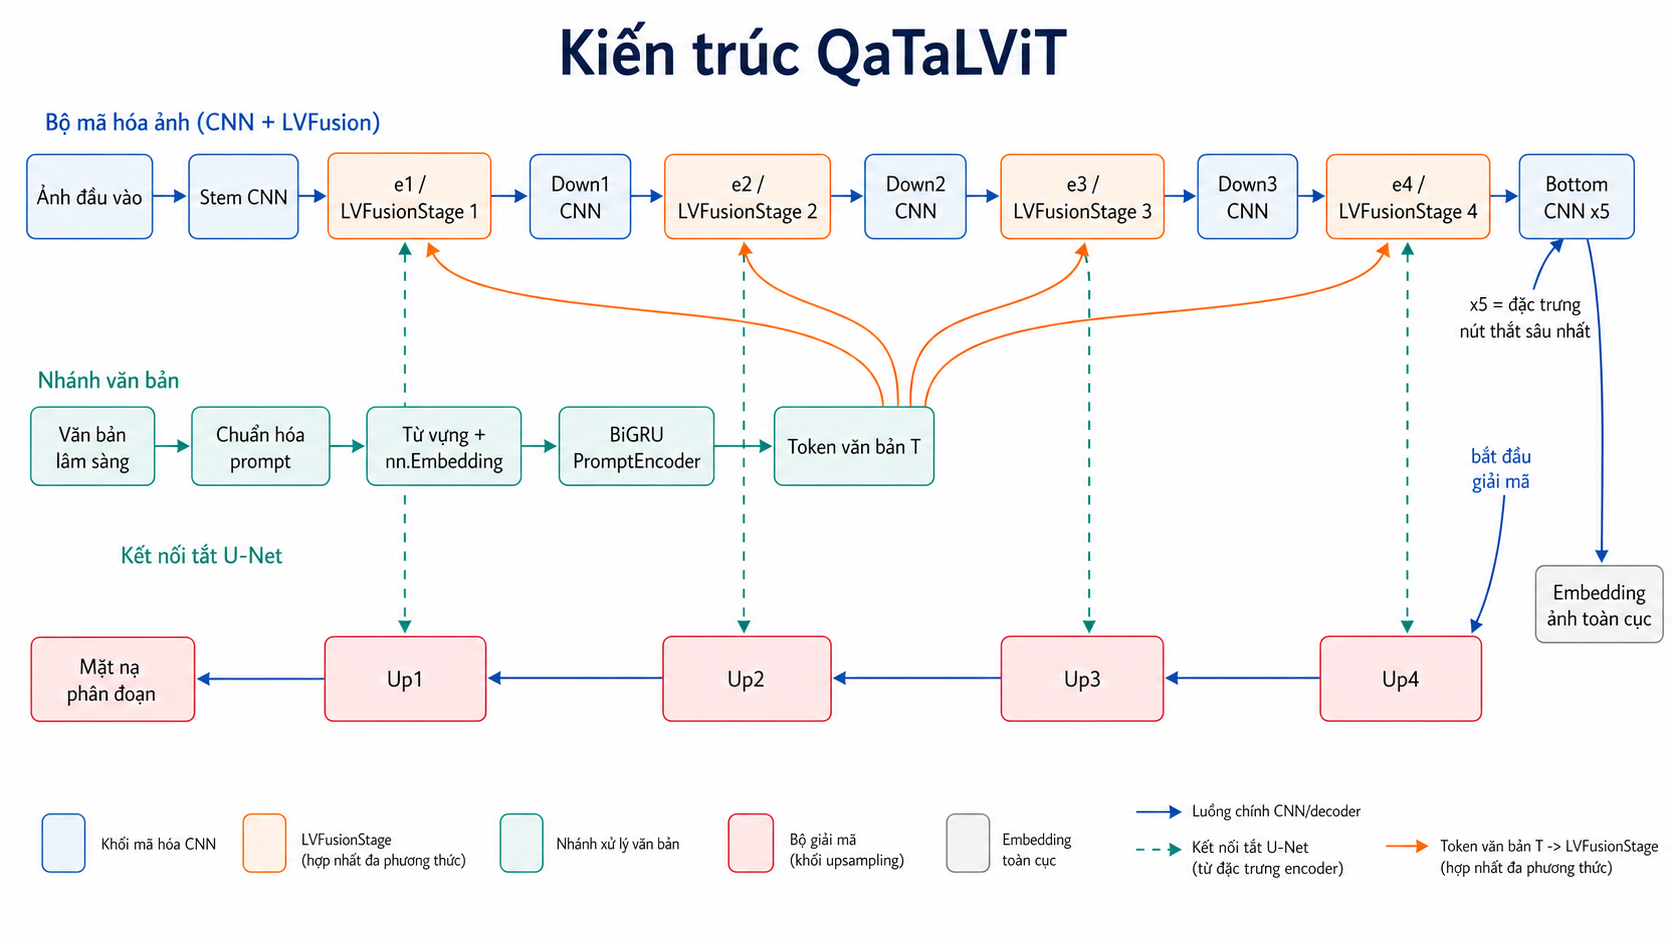
\includegraphics[width=\linewidth]{figures/qatalvit_architecture_pipeline.png}
    \vspace{0.3em}
    {\footnotesize (a) Kiến trúc tổng thể.}
  \end{minipage}
  \hfill
  \begin{minipage}[t]{0.49\textwidth}
    \centering
    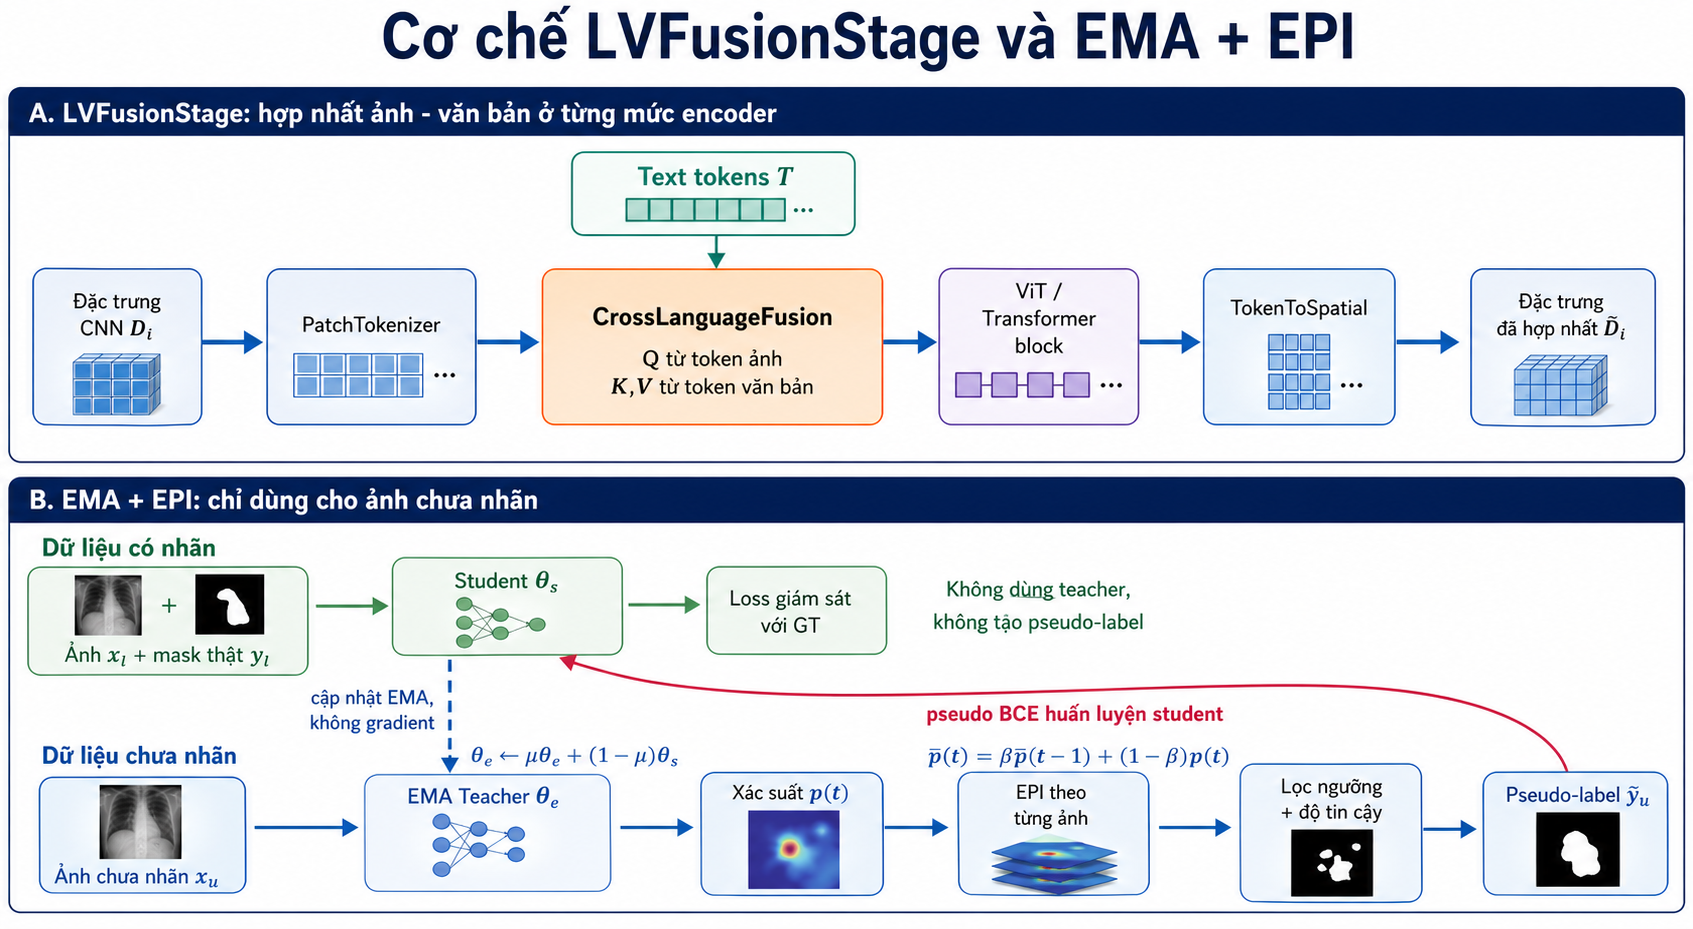
\includegraphics[width=\linewidth]{figures/qatalvit_lvfusion_ema_epi.png}
    \vspace{0.3em}
    {\footnotesize (b) Cơ chế LVFusionStage và EMA/EPI.}
  \end{minipage}
  \caption{Sơ đồ tổng quan và hai cơ chế chính của QaTaLViT.}
  \label{fig:qatalvit-pipeline}
\end{figure*}
Cho ảnh đầu vào \(x\) và văn bản văn bản đã chuẩn hóa \(t\), mô hình sinh dự đoán mặt nạ theo bốn bước: (i) ảnh được mã hóa thành đặc trưng nhiều mức bằng trục U-Net; (ii) văn bản được mã hóa bằng BiomedBERT hoặc NoBERT để tạo token văn bản và véc-tơ văn bản toàn cục; (iii) ở bốn mức mã hóa, LVFusionStage token hóa đặc trưng ảnh, thực hiện cross attention với token văn bản, rồi chiếu ngược đặc trưng đã hợp nhất về không gian ảnh; và (iv) bộ giải mã U-Net dùng các đặc trưng nối tắt đã được tinh chỉnh bởi ngôn ngữ để khôi phục mặt nạ phân đoạn cuối.

\subsection{Trục U-Net với hợp nhất ngôn ngữ đa mức}

\subsubsection{Nhánh CNN}

Trục chính của mô hình là một mạng mã hóa--giải mã kiểu U-Net. Ảnh đầu vào lần lượt đi qua các khối stem, down1, down2, down3 và bottom; bộ giải mã dùng các khối up4, up3, up2, up1 để phục hồi độ phân giải trước khi đi vào đầu phân đoạn một kênh. Với \(Y_i\) là đầu vào của một tầng tích chập, mỗi khối cơ sở có thể được mô tả dưới dạng
\[
D_i = \operatorname{GELU}\!\bigl(\operatorname{BN}_i(\operatorname{Conv}_i(Y_i))\bigr),
\]
\[
Y_{i+1} = \operatorname{Pool}(D_i),
\]
trong đó khối DoubleConv lặp lại phép biến đổi này hai lần ở mỗi mức. Bộ mã hóa--giải mã CNN giữ vai trò khung chính quyết định cấu trúc không gian của mặt nạ đầu ra.

\subsubsection{Nhánh văn bản}

Nhánh văn bản bắt đầu từ văn bản đã chuẩn hóa và có hai lựa chọn mã hóa. Ở cấu hình BiomedBERT, văn bản được đưa qua tokenizer và bộ mã hóa BiomedBERT tiền huấn luyện để tạo embedding ngữ cảnh y sinh; các embedding này sau đó được chiếu về cùng chiều đặc trưng dùng cho fusion. Ở cấu hình NoBERT, văn bản được ánh xạ thành chỉ số từ vựng nội bộ, đi qua một lớp nhúng học được và một BiGRU một lớp để tạo token văn bản. Nếu \(e_k\) là véc-tơ nhúng của token thứ \(k\), nhánh NoBERT có thể được tóm tắt bởi
\[
H = \operatorname{BiGRU}(e_1,\dots,e_L),
\]
\[
T = \operatorname{Proj}(H),
\qquad
t_{\mathrm{global}} = \frac{\sum_{k=1}^{L} m_k T_k}{\max\!\left(1,\sum_{k=1}^{L} m_k\right)},
\]
trong đó \(m_k\) là mặt nạ độ dài của văn bản. Với BiomedBERT, \(T\) được lấy từ chuỗi embedding ngữ cảnh sau phép chiếu; với NoBERT, \(T\) được lấy từ đầu ra BiGRU. Trong cả hai trường hợp, toàn bộ tín hiệu văn bản được đưa sang các tầng hợp nhất dưới dạng cùng một cặp \((T, t_{\mathrm{global}})\), gồm chuỗi token ngữ cảnh và véc-tơ toàn cục. Vì vậy, khác biệt giữa BiomedBERT và NoBERT chỉ nằm ở luồng mã hóa văn bản, còn LVFusionStage và các luồng phân đoạn phía sau là giống nhau.

\subsection{Hợp nhất ảnh--văn bản đa mức}

Ở mỗi mức mã hóa, đặc trưng ảnh được chuyển sang token bằng PatchTokenizer:
\[
x_i = \operatorname{PatchEmbed}(D_i).
\]
\noindent Sau đó, CrossLanguageFusion dùng token ảnh làm truy vấn và token văn bản làm khóa/giá trị:
\[
Q_i = \operatorname{LN}(x_i), \qquad
K_i = V_i = W_t\,\operatorname{LN}(T),
\]
\[
G_i = \sigma\!\Bigl(\operatorname{MLP}\!\bigl[\,\operatorname{LN}(x_i),\;
\operatorname{mean}(W_t\operatorname{LN}(T))\,\bigr]\Bigr),
\]
\[
X_i^{\text{cross}} = x_i + G_i \odot \operatorname{Attn}(Q_i,K_i,V_i),
\]
trong đó \(G_i\) là cổng học được từ token ảnh đã chuẩn hóa và trung bình token văn bản sau phép chiếu \(W_t\). Chuỗi token đã hợp nhất tiếp tục đi qua một số TransformerBlock, rồi được chiếu ngược về không gian ảnh bằng TokenToSpatial:
\[
\widetilde{D}_i = D_i + \operatorname{Reconstruct}\!\bigl(\operatorname{Transformer}(X_i^{\text{cross}})\bigr).
\]
Toàn bộ cơ chế này được gọi là LVFusionStage. Bốn tầng LVFusionStage được đặt tại các mức mã hóa lv1--lv4, nhờ đó văn bản có thể điều chỉnh đặc trưng ảnh từ mức biên cục bộ tới mức ngữ nghĩa sâu hơn thay vì chỉ tác động tại một điểm hợp nhất duy nhất.

\subsection{Nhánh bán giám sát với EMA teacher}

Nhánh bán giám sát dùng một mô hình teacher để tạo mục tiêu tạm thời cho dữ liệu chưa nhãn, nhưng chỉ student được cập nhật bằng gradient. Gọi \(\theta_s^{(t)}\) là tham số student tại bước \(t\) và \(\theta_e^{(t)}\) là tham số teacher, teacher được cập nhật bằng trung bình trượt hàm mũ của tham số student:
\[
\theta_e^{(t)} = \mu \theta_e^{(t-1)} + (1-\mu)\theta_s^{(t)},
\qquad \mu=0.999.
\]
EMA ở đây không tạo thêm một loss riêng, mà đóng vai trò giảm dao động của mô hình sinh nhãn giả. Nói cách khác, teacher là một phiên bản chậm hơn của student, thường ít nhạy hơn với nhiễu tức thời của từng mini-batch.

Sau khi teacher sinh xác suất \(p^{(t)}\) cho một ảnh chưa nhãn, QaTaLViT duy trì thêm một bộ nhớ dự đoán theo từng ảnh, tương tự tinh thần EPI trong LViT. Bộ nhớ này tích lũy dự đoán của cùng một mẫu qua các lần xuất hiện khác nhau:
\[
\bar{p}^{(t)} = \beta \bar{p}^{(t-1)} + (1-\beta)p^{(t)},
\qquad \beta=0.99,
\]
trong đó \(\bar{p}^{(t-1)}\) là dự đoán đã lưu ở lần trước của cùng ảnh. Như vậy, EMA hoạt động trên không gian tham số của mô hình, còn EPI hoạt động trên không gian xác suất của từng mẫu chưa nhãn. Hai cơ chế này xử lý hai nguồn nhiễu khác nhau: EMA giảm nhiễu do cập nhật trọng số, còn EPI giảm việc nhãn giả đổi đột ngột giữa các vòng huấn luyện.

Từ xác suất tích lũy \(\bar{p}\), nhãn giả và mặt nạ tin cậy được xác định bởi
\[
\bar{y}_u = \mathbf{1}(\bar{p}\ge \tau_p), \qquad
m_u = \mathbf{1}(\max(\bar{p},1-\bar{p})\ge \tau_c),
\]
trong đó \(\tau_p\) là ngưỡng tạo mặt nạ giả và \(\tau_c\) là ngưỡng độ tin cậy. Trong các cấu hình chính trên QaTa-COV19, \(\tau_p=0.5\) và \(\tau_c=0.80\). Chỉ các điểm ảnh có xác suất đủ xa khỏi biên quyết định mới được dùng trong loss chưa nhãn; các điểm ảnh còn mơ hồ bị bỏ qua. Thiết kế này giữ nhánh bán giám sát đơn giản hơn LV loss dựa trên khuôn mẫu của LViT: văn bản ảnh hưởng tới biểu diễn phân đoạn thông qua các tầng hợp nhất và thành phần căn chỉnh ở dữ liệu có nhãn, còn chất lượng nhãn giả được kiểm soát trực tiếp bằng xác suất teacher và mặt nạ tin cậy.

\subsection{Hàm mục tiêu}

Với dữ liệu có nhãn, loss giám sát chính kết hợp BCE, Dice, Focal Tversky và căn chỉnh ảnh--văn bản:
\[
\mathcal{L}_{\text{sup}} =
\lambda_{\text{bce}}\mathcal{L}_{\text{BCE}} +
\lambda_{\text{dice}}\mathcal{L}_{\text{Dice}} +
\lambda_{\text{ft}}\mathcal{L}_{\text{FT}} +
\lambda_{\text{align}}\mathcal{L}_{\text{align}}.
\]
Trong các thí nghiệm chính, các trọng số mặc định lần lượt là \(0.45\), \(0.35\), \(0.15\) và \(0.05\). Thành phần căn chỉnh được xây dựng theo kiểu CLIP đối xứng:
\[
\begin{aligned}
\mathcal{L}_{\text{align}} =
\tfrac{1}{2}\Bigl[
&\operatorname{CE}\!\left(\frac{\operatorname{norm}(z_v)\operatorname{norm}(z_t)^\top}{\tau}, I\right)\\
+\;&\operatorname{CE}\!\left(\frac{\operatorname{norm}(z_t)\operatorname{norm}(z_v)^\top}{\tau}, I\right)
\Bigr],
\end{aligned}
\]
trong đó \(z_v\) và \(z_t\) là véc-tơ nhúng toàn cục của ảnh và văn bản.

Với dữ liệu chưa nhãn, mô hình dùng một thành phần BCE nhãn giả trên các điểm ảnh thỏa \(m_u=1\):
\[
\mathcal{L}_{u} =
\lambda_p
\frac{\sum \bigl[\mathcal{L}_{\text{BCE}}(z_u,\bar{y}_u)\odot m_u\bigr]}
{\sum m_u},
\]
trong đó \(z_u\) là logit của student trên dữ liệu chưa nhãn và \(\lambda_p\) là trọng số của loss nhãn giả. Tổng loss tối ưu student là
\[
\mathcal{L} = \mathcal{L}_{\text{sup}} + \mathcal{L}_{u}.
\]
Như vậy, hàm mục tiêu của QaTaLViT kết hợp giám sát điểm ảnh trên dữ liệu có nhãn, căn chỉnh ảnh--văn bản ở mức biểu diễn và học từ dữ liệu chưa nhãn thông qua nhãn giả được lọc theo độ tin cậy. Thiết kế này giữ vai trò của văn bản trong cả học biểu diễn và học bán giám sát, nhưng vẫn kiểm soát trực tiếp nhiễu của nhãn giả bằng xác suất teacher.

\section{Thực nghiệm}
\label{sec:setup}

\subsection{Thiết lập thực nghiệm}

Các thí nghiệm được tiến hành trên hai bộ dữ liệu: QaTa-COV19 cho miền X-quang ngực và MosMedData+ cho miền CT lát cắt; thống kê số mẫu và cách chia tập đã được tóm tắt ở Bảng~\ref{tab:dataset-splits}. Theo giao thức dùng trong nghiên cứu này, 7145 ảnh của phần huấn luyện/kiểm định QaTa-COV19 được chia tiếp thành 5716 mẫu huấn luyện và 1429 mẫu kiểm định, trong khi 2113 ảnh còn lại được giữ làm tập kiểm tra độc lập. Từ tập huấn luyện, nhóm nghiên cứu tạo ba mức giám sát 25\%, 50\% và 100\% để mô phỏng lần lượt các kịch bản ít nhãn, trung bình và đủ nhãn. Với MosMedData+, nghiên cứu này dùng thiết lập mở rộng 50\% nhãn. Lựa chọn này phù hợp với mục tiêu kiểm tra các thành phần liên quan đến pseudo-label: dữ liệu có nhãn thật vẫn đủ để giữ student ổn định, nhưng dữ liệu chưa nhãn còn đủ lớn để đánh giá tác động của EMA/EPI và nhãn giả. 

QaTa-COV19 và MosMedData+ đóng hai vai trò bổ sung cho nhau. QaTa-COV19 cho phép kiểm tra chi tiết tác động của văn bản có cấu trúc trong miền X-quang, còn MosMedData+ cho thấy mô hình và recipe huấn luyện phản ứng thế nào khi chuyển sang CT có lệch miền mạnh hơn. Vì vậy, kết quả MosMedData+ được đưa vào bảng chính và phần phân tích riêng, thay vì chỉ được xem như ghi chú phụ.

Về mã hóa văn bản, các thí nghiệm của QaTaLViT được chia thành hai lựa chọn cấu hình. Cấu hình BiomedBERT dùng bộ mã hóa ngôn ngữ y sinh tiền huấn luyện để sinh biểu diễn văn bản, sau đó chiếu về không gian đặc trưng dùng chung cho LVFusionStage. Cấu hình NoBERT bỏ bộ mã hóa tiền huấn luyện và thay bằng từ vựng học được, lớp nhúng và BiGRU nhẹ. Hai cấu hình này dùng cùng ảnh đầu vào, cùng trục U-Net, cùng bốn tầng LVFusionStage, cùng decoder và cùng hàm loss; vì vậy các so sánh BiomedBERT--NoBERT trong phần kết quả chủ yếu phản ánh tác động của riêng luồng mã hóa văn bản.

\subsection{Thước đo đánh giá}

Hai thước đo chính là Dice và mIoU. Đây cũng là hai thước đo được LViT sử dụng để đánh giá cả so sánh chính lẫn phân tích loại bỏ thành phần, do chúng phản ánh tốt đồng thời mức chồng lấp tổng thể và chất lượng phân đoạn trên bài toán tổn thương y khoa \cite{li2023lvit}. Trong nghiên cứu này, mIoU được dùng theo nghĩa IoU của lớp tổn thương lấy trung bình theo mẫu. Với dự đoán \(\hat{y}_i\) và nhãn thật \(y_i\) của mẫu thứ \(i\), Dice được hiểu như hệ số chồng lấp trung bình theo mẫu:
\[
\mathrm{Dice} =
\frac{1}{N}\sum_{i=1}^{N}
\frac{2|\hat{y}_i\cap y_i|}{|\hat{y}_i|+|y_i|},
\]
trong khi mIoU được tính dưới dạng IoU của lớp tổn thương lấy trung bình theo mẫu:
\[
\mathrm{mIoU} = \frac{1}{N}\sum_{i=1}^{N}\frac{|\hat{y}_i\cap y_i|}{|\hat{y}_i\cup y_i|}.
\]
Ngoài chỉ số cuối trên tập kiểm tra, nhóm nghiên cứu còn theo dõi vòng kiểm định tốt nhất để chọn mô hình tốt nhất sau khi huấn luyện xong mô hình, Dice/mIoU kiểm định tốt nhất và chất lượng nhãn giả trên tập giữ lại ở các cấu hình 25\% và 50\% nhãn.

\subsection{Chi tiết cài đặt}

Các thí nghiệm chính dùng ảnh đầu vào kích thước \(224\times224\), 60 vòng huấn luyện, cỡ lô 16 trên mỗi GPU và cỡ lô hiệu dụng mục tiêu 16. Bộ tối ưu hóa dùng tốc độ học \(3\times10^{-4}\), suy giảm trọng số \(10^{-4}\), bộ điều phối cosine có làm nóng, seed 42 và hệ số EMA 0.999. Mô hình được chọn theo mốc lưu tốt nhất trên tập kiểm định; trong các thí nghiệm chính, mốc tốt nhất thường xuất hiện ở khoảng vòng 37--43, cho thấy mô hình hội tụ tương đối sớm sau khi tín hiệu teacher trở nên ổn định.

Trong phần so sánh, nhóm nghiên cứu sử dụng hai tầng mốc đối chiếu. Tầng thứ nhất là LViT được huấn luyện lại theo đúng giao thức chia nhãn và đánh giá của nghiên cứu này; đây là tầng so sánh công bằng nhất để đo tác động thực sự của các thay đổi kiến trúc. Tầng thứ hai là các mốc đã công bố trong bài báo LViT \cite{li2023lvit}; các mốc này không thay thế cho đối chứng nội bộ, nhưng cung cấp bối cảnh học thuật rộng hơn cho các bảng so sánh bán giám sát và giám sát đầy đủ.

\subsection{So sánh với các phương pháp đối sánh}

\begin{figure*}[!t]
  \centering
  
\includegraphics[width=0.32\textwidth]{qata25_analysis/qata25_combined_curves.png}\hfill
  
\includegraphics[width=0.32\textwidth]{qata50_analysis/qata50_combined_curves.png}\hfill
  
\includegraphics[width=0.32\textwidth]{qata100_analysis/qata100_combined_curves.png}
  \caption{Đường cong huấn luyện ở ba mức nhãn.}
  \label{fig:train-curves}
\end{figure*}

\begin{figure*}[!t]
  \centering
  
\includegraphics[width=0.47\textwidth]{qata25_analysis/qata25_pseudo_quality.png}\hfill
  
\includegraphics[width=0.47\textwidth]{qata50_analysis/qata50_pseudo_quality.png}
  \caption{Chất lượng nhãn giả ở hai cấu hình ít nhãn.}
  \label{fig:pseudo-quality}
\end{figure*}


\begin{table*}[!t]
  \centering
  \caption{So sánh với các phương pháp đối sánh trên QaTa-COV19 và MosMedData+.}
  \label{tab:main-results}
  \resizebox{\textwidth}{!}{%
  \begin{tabular}{cccccccccc}
    \midrule
    \multicolumn{1}{c}{} &
    \multicolumn{1}{c}{} &
    &&&&
    \multicolumn{2}{c}{\textbf{QaTa-COV19}} &
    \multicolumn{2}{c}{\textbf{MosMedData+}} \\
    \cmidrule(r){7-8}\cmidrule(l){9-10}
    \multicolumn{1}{c}{\textbf{Phương pháp}} &
    \textbf{Backbone} &
    \textbf{Text} &
    \textbf{Tỉ lệ nhãn} &
    \textbf{Param (M)} &
    \textbf{FLOPs (G)} &
    Dice (\%) & mIoU (\%) & Dice (\%) & mIoU (\%) \\
    \hline
    \rowcolor{black!10} U-Net & CNN & $\times$ & 100\% & 14.8 & 50.3 & 79.02 & 69.46 & 64.60 & 50.73 \\
    \rowcolor{black!10} UNet++ & CNN & $\times$ & 100\% & 74.5 & 94.6 & 79.62 & 70.25 & 71.75 & 58.39 \\
    \rowcolor{black!10} AttUNet & CNN & $\times$ & 100\% & 34.9 & 101.9 & 79.31 & 70.04 & 66.34 & 52.82 \\
    \rowcolor{black!10} nnUNet & CNN & $\times$ & 100\% & 19.1 & 412.7 & 80.42 & 70.81 & 72.59 & 60.36 \\
    \rowcolor{black!10} TransUNet & Hybrid & $\times$ & 100\% & 105.0 & 56.7 & 78.63 & 69.13 & 71.24 & 58.44 \\
    \rowcolor{black!10} Swin-Unet & Hybrid & $\times$ & 100\% & 82.3 & 67.3 & 78.07 & 68.34 & 63.29 & 50.19 \\
    \rowcolor{black!10} UCTransNet & Hybrid & $\times$ & 100\% & 65.6 & 63.2 & 79.15 & 69.60 & 65.90 & 52.69 \\
    \hline
    \rowcolor{black!15} \textbf{LViT-TW (1/4)} & Hybrid & $\times$ & 25\% & 28.0 & 54.0 & 79.08 & 69.42 & 70.65 & 58.07 \\
    \rowcolor{black!15} \textbf{LViT-TW (1/2)} & Hybrid & $\times$ & 50\% & 28.0 & 54.0 & 80.35 & 70.74 & 71.89 & 59.63 \\
    \rowcolor{black!15} \textbf{LViT-TW} & Hybrid & $\times$ & 100\% & 28.0 & 54.0 & 81.12 & 71.37 & 72.58 & 60.40 \\
    \hline
    \rowcolor{yellow!10} ConVIRT & CNN & $\checkmark$ & 100\% & 35.2 & 44.6 & 79.72 & 70.58 & 72.06 & 59.73 \\
    \rowcolor{yellow!10} TGANet & CNN & $\checkmark$ & 100\% & 19.8 & 41.9 & 79.87 & 70.75 & 71.81 & 59.28 \\
    \rowcolor{yellow!10} CLIP & Hybrid & $\checkmark$ & 100\% & 87.0 & 105.3 & 79.81 & 70.66 & 71.97 & 59.64 \\
    \rowcolor{yellow!10} GLoRIA & Hybrid & $\checkmark$ & 100\% & 45.6 & 60.8 & 79.94 & 70.68 & 72.42 & 60.18 \\
    \rowcolor{yellow!10} ViLT & Hybrid & $\checkmark$ & 100\% & 87.4 & 55.9 & 79.63 & 70.12 & 72.36 & 60.15 \\
    \rowcolor{yellow!10} LAVT & Hybrid & $\checkmark$ & 100\% & 118.6 & 83.8 & 79.28 & 69.89 & 73.29 & 60.41 \\
    \hline
    \rowcolor{yellow!15} \textbf{LViT-T (1/4)} & Hybrid & $\checkmark$ & 25\% & 29.7 & 54.1 & 80.95 & 71.31 & 72.48 & 60.31 \\
    \rowcolor{yellow!15} \textbf{LViT-T (1/2)} & Hybrid & $\checkmark$ & 50\% & 29.7 & 54.1 & 82.73 & 73.99 & 73.56 & 61.05 \\
    \rowcolor{yellow!15} \textbf{LViT-T} & Hybrid & $\checkmark$ & 100\% & 29.7 & 54.1 & 83.66 & 75.11 & 74.57 & 61.33 \\
    \hline
    \rowcolor{blue!8} \textbf{QaTaLViT (1/4)} & Hybrid & $\checkmark$ & 25\% & 32.3 & 67.8 & \textbf{82.22} & \textbf{73.35} & \multicolumn{2}{c}{--} \\
    \rowcolor{blue!8} \textbf{QaTaLViT (1/2)} & Hybrid & $\checkmark$ & 50\% & 32.3 & 67.8 & \textbf{84.03} & \textbf{75.62} & \textbf{73.84} & \textbf{60.31} \\
    \rowcolor{blue!8} \textbf{QaTaLViT} & Hybrid & $\checkmark$ & 100\% & 32.3 & 67.8 & \textbf{85.28} & \textbf{77.25} & \multicolumn{2}{c}{--} \\
    \hline
  \end{tabular}%
  }
\tablenotesep
\begin{minipage}{0.98\textwidth}
\scriptsize
Các mốc đối sánh không phải QaTaLViT được trích từ bản công bố chính thức của LViT \cite{li2023lvit}. Dấu -- trong các hàng QaTaLViT của cột MosMedData+ biểu thị cấu hình không thuộc phạm vi thí nghiệm mở rộng 50\% của báo cáo.
\end{minipage}
\end{table*}

Bảng~\ref{tab:main-results} so sánh đồng thời backbone, việc dùng văn bản, tỉ lệ nhãn, chi phí mô hình và kết quả trên hai bộ dữ liệu. Trên QaTa-COV19, QaTaLViT đạt kết quả cao nhất ở cả ba mức nhãn. So với LViT-T được công bố, mô hình tăng 1.27 điểm Dice ở 25\% nhãn, 1.30 điểm Dice ở 50\% nhãn và 1.62 điểm Dice ở 100\% nhãn. Đáng chú ý, cấu hình 50\% nhãn của QaTaLViT đạt 84.03\% Dice và 75.62\% mIoU, vượt mốc LViT-T 100\% nhãn trên cùng bảng tham chiếu.

Trên MosMedData+, báo cáo dùng thiết lập 50\% nhãn như một thí nghiệm mở rộng có kiểm soát. Biến thể QaTaLViT tốt nhất hiện tại dùng BiomedBERT, tắt EMA/EPI và tăng cường nhẹ bằng biến đổi affine và elastic deformation đạt 73.84\% Dice và 60.31\% mIoU sau khi tinh chỉnh ngưỡng. So với LViT-T 50\% được công bố là 73.56\%/61.05\%, kết quả này vượt 0.28 điểm Dice nhưng vẫn thấp hơn 0.74 điểm mIoU. Điều này cho thấy hướng cải thiện trên MosMedData+ đã bắt đầu vượt được mốc Dice của LViT ở cùng mức nhãn.

\begin{table}[!t]
  \centering
  \caption{So sánh bán giám sát trên QaTa-COV19.}
  \label{tab:semi-supervised-results}
  \resizebox{\columnwidth}{!}{%
  \small
  \begin{tabular}{ccccc}
    \toprule
    \textbf{Phương pháp} & Text & Tỉ lệ nhãn & \textbf{Dice (\%)} & \textbf{mIoU (\%)} \\
    \midrule
    DTC & $\times$ & 25\% & 76.07 & 66.04 \\
    PLCT & $\times$ & 25\% & 76.65 & 66.71 \\
    MC-Net+ & $\times$ & 25\% & 76.93 & 67.02 \\
    LViT-TW (1/4) & $\times$ & 25\% & 79.08 & 69.42 \\
    \midrule
    LAVT & $\checkmark$ & 25\% & 77.08 & 67.21 \\
    GLoRIA & $\checkmark$ & 25\% & 77.32 & 67.48 \\
    LViT-T (1/4) & $\checkmark$ & 25\% & 80.95 & 71.31 \\
    \textbf{QaTaLViT} & $\checkmark$ & 25\% & \textbf{82.22} & \textbf{73.35} \\
    \midrule
    DTC & $\times$ & 50\% & 77.23 & 67.42 \\
    PLCT & $\times$ & 50\% & 77.66 & 68.04 \\
    MC-Net+ & $\times$ & 50\% & 77.91 & 68.47 \\
    LViT-TW (1/2) & $\times$ & 50\% & 80.35 & 70.74 \\
    \midrule
    LAVT & $\checkmark$ & 50\% & 77.96 & 68.53 \\
    GLoRIA & $\checkmark$ & 50\% & 78.49 & 68.97 \\
    LViT-T (1/2) & $\checkmark$ & 50\% & 82.73 & 73.99 \\
    \textbf{QaTaLViT} & $\checkmark$ & 50\% & \textbf{84.03} & \textbf{75.62} \\
    \bottomrule
  \end{tabular}%
  }
\end{table}

Bảng~\ref{tab:semi-supervised-results} tách riêng thiết lập bán giám sát. Ở 25\% nhãn, QaTaLViT vượt LViT-T (1/4) 1.27 điểm Dice và 2.04 điểm mIoU; ở 50\% nhãn, mô hình vượt LViT-T (1/2) 1.30 điểm Dice và 1.63 điểm mIoU. So với các phương pháp bán giám sát không văn bản như DTC, PLCT và MC-Net+, khoảng cách còn lớn hơn, cho thấy văn bản chuẩn hóa và hợp nhất đa mức đóng vai trò đặc biệt rõ trong kịch bản ít nhãn.

\subsection{Phân tích động học huấn luyện}

Ở 25\% nhãn, vòng kiểm định tốt nhất là 37 với Dice/mIoU kiểm định 80.09\%/70.17\%; ở 50\% nhãn, vòng tốt nhất là 43 với Dice/mIoU kiểm định 81.49\%/71.80\%; còn cấu hình 100\% nhãn cũng đạt vòng tốt nhất quanh 43 với 82.86\%/73.52\%. Riêng cấu hình 50\% nhãn có nhãn giả trung bình 82.34\% Dice và 73.00\% mIoU, rất gần với chất lượng kiểm định tương ứng. Điều đó cho thấy teacher EMA cùng cơ chế EPI và mặt nạ tin cậy đang giúp giữ chất lượng nhãn giả đủ ổn định, chứ không chỉ làm tăng số lượng điểm ảnh được dùng làm giám sát giả. Ở 25\% nhãn, khoảng cách giữa huấn luyện và kiểm định còn rộng hơn, cho thấy mô hình vẫn chịu áp lực quá khớp mạnh khi số mặt nạ thật quá ít.

Hình~\ref{fig:train-curves} và Hình~\ref{fig:pseudo-quality} đóng vai trò hình định tính/động học, sử dụng để giải thích cơ chế cải thiện. Ở 25\% nhãn, Dice huấn luyện cuối xấp xỉ 95.9\% trong khi kiểm định chỉ quanh 80.1\%, biểu hiện rõ hiện tượng mô hình học quá nhanh trên tập nhãn nhỏ. Ở 50\% nhãn, khoảng cách này thu hẹp đáng kể và đồng thời chất lượng nhãn giả cũng tăng lên. Nói cách khác, 50\% là điểm mà cả hai nhánh -- có giám sát và bán giám sát -- cùng hoạt động ổn định.

\subsection{Phân tích loại bỏ thành phần}

\label{sec:ablation}

\subsubsection{Ablation thành phần chính trên QaTa-COV19}

\begin{table*}[!t]
  \centering
  \caption{Ablation thành phần trên QaTa-COV19.}
  \label{tab:ablation}
  \scriptsize
  \renewcommand{\arraystretch}{1.14}
  \setlength{\tabcolsep}{2.5pt}
  \begin{tabularx}{\textwidth}{@{}lcccccccYYY@{}}
    \toprule
    Phương pháp & SSL mới & Prompt & Tăng & 4-LVF & FT & Căn chỉnh & Recipe cuối & 25\% nhãn & 50\% nhãn & 100\% nhãn \\
    \midrule
    Mốc nền (LViT) & -- & -- & -- & -- & -- & -- & -- & 78.42 / 68.43 & 80.32 / 70.60 & 83.06 / 74.08 \\
    B0 & \(\checkmark\) & -- & -- & -- & -- & -- & -- & 77.49 / 67.19 & 79.54 / 69.71 & 82.76 / 73.78 \\
    I1 & \(\checkmark\) & \(\checkmark\) & -- & -- & -- & -- & -- & 78.46 / 68.23 & 80.89 / 71.54 & 82.84 / 74.14 \\
    I2 & \(\checkmark\) & \(\checkmark\) & \(\checkmark\) & -- & -- & -- & -- & 80.45 / 71.04 & 82.61 / 73.65 & 83.69 / 74.85 \\
    I3 & \(\checkmark\) & \(\checkmark\) & \(\checkmark\) & \(\checkmark\) & -- & -- & -- & 78.96 / 69.22 & 82.61 / 73.64 & 83.05 / 74.45 \\
    I4 & \(\checkmark\) & \(\checkmark\) & \(\checkmark\) & \(\checkmark\) & \(\checkmark\) & -- & -- & 81.37 / 72.10 & 82.51 / 73.54 & 83.75 / 75.03 \\
    I5 & \(\checkmark\) & \(\checkmark\) & \(\checkmark\) & \(\checkmark\) & \(\checkmark\) & \(\checkmark\) & -- & 80.24 / 70.57 & 82.94 / 74.10 & 83.67 / 74.97 \\
    QaTaLViT & \(\checkmark\) & \(\checkmark\) & \(\checkmark\) & \(\checkmark\) & \(\checkmark\) & \(\checkmark\) & \(\checkmark\) & \textbf{82.22 / 73.35} & \textbf{84.03 / 75.62} & \textbf{85.28 / 77.25} \\
    \bottomrule
  \end{tabularx}
\tablenotesep
\begin{minipage}{0.98\textwidth}
\scriptsize
\textit{Ghi chú.} SSL mới: EMA/EPI với BCE nhãn giả thay cho LV loss khuôn mẫu.
Prompt: chuẩn hóa văn bản.
Tăng: tăng cường dữ liệu an toàn.
4-LVF: bốn tầng LVFusionStage.
FT: Focal Tversky.
Căn chỉnh: thêm hàm mất mát căn chỉnh ảnh--văn bản.
Recipe cuối: công thức huấn luyện đã khóa cho bản hoàn chỉnh.
Mỗi ô kết quả là Dice / mIoU (\%).
\end{minipage}
\end{table*}

Chuỗi trong Bảng~\ref{tab:ablation} bắt đầu từ mô hình nền, bỏ dần phụ thuộc vào LV loss/khuôn mẫu cứng, rồi bổ sung các cơ chế mềm hơn để kiểm soát nhãn giả và khai thác văn bản. Vì các biến thể trung gian là chuỗi tích lũy, bảng nên được đọc như quá trình thay thế từng phần của LViT, không phải như tập hợp các mô-đun độc lập hoàn toàn.

Trước hết, B0 cho thấy chỉ riêng việc bỏ LV loss/khuôn mẫu cứng mà chưa có cơ chế thay thế đủ mạnh có thể làm hiệu năng giảm ở 25\% và 50\% nhãn. Điều này rất quan trọng: điểm yếu của LViT không nằm ở chỗ đưa văn bản vào bài toán, mà ở chỗ văn bản bị buộc phải đóng vai trò một khuôn mẫu giám sát quá cứng. Khi thêm I1 và đặc biệt là I2, mô hình bắt đầu phục hồi và vượt mốc nền, cho thấy việc thay nhánh hợp nhất cũ bằng hợp nhất ảnh--văn bản đa mức là một thay đổi đúng hướng.

Tiếp theo, chuỗi I3--I5 cho thấy cải thiện cuối cùng có xu hướng là hiệu ứng toàn hệ thống, không phải kết quả của một thành phần đơn lẻ. Ở 25\% nhãn, mốc trung gian tốt nhất đạt 81.37\% Dice, nhưng bản hoàn chỉnh đạt 82.22\%. Ở 50\% và 100\% nhãn, khoảng cách này lần lượt là 1.09 và 1.53 điểm Dice. Nói cách khác, hợp nhất đa mức bằng LVFusionStage, Focal Tversky và căn chỉnh ảnh--văn bản nhiều khả năng chỉ phát huy hết khi được phối hợp trong cùng một hệ.

Cuối cùng, mức tăng vẫn tồn tại rõ ở 100\% nhãn, tức trong thiết lập mà dữ liệu chưa nhãn không còn tham gia. Quan sát này cho phép kết luận rằng QaTaLViT không chỉ là một kỹ thuật bán giám sát, mà là một kiến trúc phân đoạn tốt hơn ngay cả khi mức giám sát đã đầy đủ. Đây cũng là điểm khác quan trọng khi đối chiếu với cách LViT trình bày thí nghiệm: các thay đổi của QaTaLViT vừa cải thiện nhánh chưa nhãn, vừa cải thiện trực tiếp nhánh phân đoạn có giám sát.

\newpage

\subsubsection{Ablation siêu tham số trên QaTa-COV19}
\label{sec:hyperparameter-ablation}

Bảng~\ref{tab:hyperparameter-ablation} tóm tắt các thay đổi siêu tham số chính trên cấu hình QaTa-COV19 50\% nhãn, nhằm kiểm tra liệu recipe cuối có ổn định trước learning rate và effective batch size hay không.

\begin{table}[H]
  \centering
  \caption{Ablation siêu tham số trên QaTa-COV19.}
  \label{tab:hyperparameter-ablation}
  \footnotesize
  \renewcommand{\arraystretch}{1.24}
  \setlength{\tabcolsep}{3pt}
  \begin{tabularx}{\columnwidth}{@{}>{\raggedright\arraybackslash}p{0.27\columnwidth} L >{\centering\arraybackslash}p{0.25\columnwidth}@{}}
    \toprule
    Biến thể & Thay đổi chính & Dice / mIoU (\%) \\
    \midrule
    Recipe chuẩn & Effective batch size 32,\newline lr = \(3\times10^{-4}\) & \textbf{84.03 / 75.62} \\
    LR 1e-3 & Effective batch size 32,\newline lr = \(1\times10^{-3}\)  & 82.55 / 73.76 \\
    LR 1e-4 & Effective batch size 32,\newline lr = \(1\times10^{-4}\)  & 83.57 / 74.99 \\
    Global batch 16 & Effective batch size 16,\newline lr = \(3\times10^{-4}\)  & 83.63 / 75.18 \\
    Global batch 32 & Effective batch size 32,\newline lr = \(3\times10^{-4}\)  & 83.66 / 75.09 \\
    \bottomrule
  \end{tabularx}
\tablenotesep
\begin{minipage}{0.98\columnwidth}
\scriptsize
Mỗi ô kết quả là Dice / mIoU (\%). Các thí nghiệm trong bảng giữ cùng thiết lập QaTa-COV19 50\% nhãn và chỉ thay đổi nhóm siêu tham số được ghi ở cột thứ hai.
\end{minipage}
\end{table}

Các kết quả này cho thấy công thức cuối không chỉ tốt nhờ một lần chọn ngẫu nhiên siêu tham số. Khi tăng learning rate lên \(1\times10^{-3}\), Dice kiểm tra giảm từ 84.03\% xuống 82.55\%, cho thấy QaTa-COV19 nhạy với bước học quá lớn. Ngược lại, \(1\times10^{-4}\) giữ kiểm định khá gần cấu hình chuẩn nhưng kiểm tra vẫn thấp hơn, phù hợp với khả năng hội tụ chậm hơn. Hai thí nghiệm batch ablation với global batch 16 và 32 dao động rất nhỏ quanh 83.6\% Dice kiểm tra, nghĩa là batch size có ảnh hưởng nhưng không tạo mức tăng vượt cấu hình đã chốt. Vì vậy, các kết quả này củng cố lựa chọn giữ learning rate \(3\times10^{-4}\) và cấu hình BiomedBERT 50\% hiện tại cho kết quả chính.

\subsubsection{Ablation thiết lập huấn luyện trên MosMedData+}
\label{sec:mosmed-training-ablation}

Trong khi QaTa-COV19 cho thấy xu hướng cải thiện khá ổn định, MosMedData+ nhạy hơn với ngưỡng suy luận, tiền xử lý, nhãn giả và công thức loss. Vì vậy, bên cạnh bảng kết quả MosMedData+, nhóm nghiên cứu ghi lại một ablation thiết lập huấn luyện trên MosMedData+ ở mức 50\% nhãn. Bảng~\ref{tab:mosmed-training-ablation} chỉ sử dụng các thí nghiệm đã hoàn tất, nhằm tránh đưa các biến thể chưa có số vào phần kết quả chính.

\begin{table}[H]
  \centering
  \caption{Ablation thiết lập trên MosMedData+.}
  \label{tab:mosmed-training-ablation}
  \scriptsize
  \renewcommand{\arraystretch}{1.26}
  \setlength{\tabcolsep}{3pt}
  \begin{tabularx}{\columnwidth}{@{}>{\raggedright\arraybackslash}p{0.39\columnwidth}>{\centering\arraybackslash}p{0.22\columnwidth}X@{}}
    \toprule
    Biến thể  & Dice / mIoU (\%) & Nhận xét \\
    \midrule
    BiomedBERT ban đầu   & 68.88 / 55.14 & Teacher và pseudo chưa ổn định \\
    BiomedBERT, thêm tiền xử lý   & 70.36 / 56.97 & Thêm tiền xử lý crop bỏ background \\
    BiomedBERT, tiền xử lý, tắt EMA/EPI  & 71.88 / 58.00 & Tắt pseudo/EMA giảm nhiễu trên MosMedData+ \\
    NoBERT, tiền xử lý, tắt EMA/EPI  & \textbf{72.69 / 58.99} & Thử nghiệm với NoBERT \\
    BiomedBERT, tiền xử lý, tắt EMA/EPI, augmentation nhẹ & \textbf{73.84 / 60.31} & Kết quả MosMedData+ tốt nhất hiện tại \\
    NoBERT, tiền xử lý, tắt EMA/EPI, augmentation nhẹ & \textbf{72.77 / 59.22} & Thử nghiệm với NoBERT + augmentation nhẹ \\
    \bottomrule
  \end{tabularx}
\tablenotesep
\begin{minipage}{0.98\columnwidth}
\scriptsize
\textit{Ghi chú.} Tất cả các hàng dùng 50\% nhãn trên MosMedData+. Tiền xử lý chỉ cấu hình crop phổi/bỏ nền; tắt EMA/EPI tương ứng student-only, không dùng pseudo-label trong huấn luyện. Augmentation nhẹ là biến thể tăng cường dữ liệu nhẹ bằng biến đổi affine và elastic deformation.
\end{minipage}
\end{table}

Bảng~\ref{tab:mosmed-training-ablation} cho thấy vấn đề chính của MosMedData+ không nằm ở một thành phần kiến trúc đơn lẻ mà ở động học huấn luyện. Trong các thí nghiệm ban đầu, EMA teacher không đóng vai trò teacher mạnh hơn student như kỳ vọng: Dice của nhánh EMA thấp hơn student rõ rệt, và nhiều thời điểm xác suất đầu ra của teacher bị lệch về vùng rất thấp. Khi các xác suất này được dùng để sinh nhãn giả, confidence mask dễ giữ lại phần lớn điểm ảnh nền thay vì các điểm ảnh tổn thương. Nói cách khác, pseudo-label không chỉ nhiễu ngẫu nhiên, mà còn có thiên lệch hệ thống về nhãn âm. Với tổn thương nhỏ trong MosMedData+, thiên lệch này đặc biệt nguy hiểm: pseudo BCE trên dữ liệu chưa nhãn có thể thưởng cho mô hình khi dự đoán nền rộng hơn, làm xác suất vùng tổn thương bị nén xuống và khiến ngưỡng suy luận phải hạ thấp bất thường.

Vì vậy, việc chuyển sang tắt EMA/EPI không phải là bỏ qua bán giám sát một cách tùy tiện, mà là một bước cô lập nguyên nhân. Khi tắt EMA/pseudo, mô hình chỉ còn học từ nhãn thật và hàm mất mát được kiểm soát trực tiếp; nhờ đó, gradient không còn bị nhánh teacher yếu kéo về nền. Sau khi kết hợp tắt EMA/EPI, tiền xử lý và hiệu chỉnh ngưỡng, kết quả tăng từ 68.88\% lên 71.88--72.69\% Dice trong các thí nghiệm kiểm định. Khi bổ sung tăng cường nhẹ dùng biển đổi affine và elastic deformation ở cấu hình BiomedBERT student-only, kết quả tốt nhất tăng tiếp lên 73.84\% Dice và 60.31\% mIoU. Điều này cho thấy với tập dữ liệu có lệch miền mạnh như MosMedData+, một student được huấn luyện ổn định cùng augmentation vừa phải có thể cạnh tranh trực tiếp với mốc LViT-T 50\% đã công bố.

\subsubsection{Ablation mã hóa văn bản}
\label{sec:text-encoding}

Một kết luận thú vị khi đối chiếu với LViT là bài báo nguồn đã chỉ ra rằng lớp nhúng đơn giản có thể hiệu quả hơn bộ mã hóa văn bản nặng trên báo cáo có cấu trúc \cite{li2023lvit}. Kết quả của QaTaLViT không phủ nhận nhận định này. Ngược lại, chúng củng cố nó theo một hướng cụ thể hơn: điều quan trọng không phải là tăng năng lực xử lý ngôn ngữ tự nhiên thuần túy, mà là chuẩn hóa văn bản và đưa tín hiệu văn bản vào đúng vị trí của mạng thông qua các tầng hợp nhất đa mức. Nếu thiếu các ràng buộc đó, thêm bộ mã hóa ngôn ngữ mạnh hơn khó chuyển thành mức tăng định lượng rõ ràng cho phân đoạn.

\begin{table*}[!t]
  \centering
  \caption{Ablation mã hóa văn bản trong QaTaLViT.}
  \label{tab:qatalvit-text-encoder-ablation}
  \scriptsize
  \renewcommand{\arraystretch}{1.14}
  \setlength{\tabcolsep}{4pt}
  \begin{tabularx}{\textwidth}{@{}l L L Y Y@{}}
    \toprule
    Phương pháp & Cách mã hóa văn bản & Dạng văn bản & QaTa Dice / mIoU (\%) & MosMed Dice / mIoU (\%) \\
    \midrule
    B0 & Cách biểu diễn văn bản gần LViT & Chưa chuẩn hóa văn bản & 79.54 / 69.71 & -- \\
    I1 & Chuẩn hóa văn bản & Prompt chuẩn hóa, cùng khung B0 & 80.89 / 71.54 & -- \\
    QaTaLViT & BiomedBERT tiền huấn luyện & Prompt chuẩn hóa, chỉ thay text encoder & \textbf{84.03 / 75.62} & 72.85 / 59.41 \\
    QaTaLViT & NoBERT: lớp nhúng + BiGRU & Prompt chuẩn hóa, chỉ thay text encoder & 83.76 / 75.28 & \textbf{72.99 / 59.48} \\
    \bottomrule
  \end{tabularx}
\tablenotesep
\begin{minipage}{0.98\textwidth}
\scriptsize
\textit{Ghi chú.} Dấu -- biểu thị chưa có thí nghiệm MosMedData+ tương ứng. B0 dùng cách biểu diễn văn bản giống LViT, chưa áp dụng bước chuẩn hóa văn bản. I1 giữ cùng khung biểu diễn của B0 nhưng thay đầu vào bằng văn bản đã chuẩn hóa, nhằm tách riêng tác động của bước chuẩn hóa văn bản. Hai hàng QaTaLViT cuối dùng cùng kiến trúc phía sau text encoder: U-Net, bốn tầng LVFusionStage, decoder và loss; điểm khác nhau chỉ nằm ở cách mã hóa văn bản. BiomedBERT dùng bộ mã hóa y sinh tiền huấn luyện để tạo embedding ngữ cảnh, còn NoBERT dùng lớp nhúng và BiGRU nhẹ.
\end{minipage}
\end{table*}

Bảng~\ref{tab:qatalvit-text-encoder-ablation} kiểm tra trực tiếp liệu bài học từ LViT có còn đúng trong QaTaLViT hay không. Hai hàng B0 và I1 là mốc phụ từ chuỗi ablation QaTa-COV19 ở mức 50\% nhãn: khi chuyển từ cách biểu diễn văn bản gần LViT sang chuẩn hóa văn bản, Dice tăng từ 79.54\% lên 80.89\% và mIoU tăng từ 69.71\% lên 71.54\%. Hai hàng QaTaLViT cuối là so sánh text encoder trực tiếp: BiomedBERT và NoBERT chỉ khác nhau ở cách biến văn bản thành token văn bản trước LVFusionStage. Trên QaTa-COV19, NoBERT đạt 83.76\% Dice, rất gần với BiomedBERT 84.03\% Dice, cho thấy văn bản có cấu trúc đã mang phần lớn tín hiệu cần thiết; BiomedBERT vẫn nhỉnh hơn nhẹ trong thiết lập 50\% nhãn. Trên MosMedData+, xu hướng đảo chiều nhẹ: NoBERT đạt 72.99\% Dice và 59.48\% mIoU, cao hơn BiomedBERT 72.85\% Dice và 59.41\% mIoU trong cấu hình tắt EMA/EPI và tiền xử lý. Điều này củng cố nhận định rằng với mô tả y khoa ngắn và có cấu trúc, chuẩn hóa văn bản có thể quan trọng hơn việc dùng một bộ mã hóa ngôn ngữ nặng hơn.

Từ góc nhìn QaTaLViT, bảng này cũng giúp diễn giải ablation trong Bảng~\ref{tab:ablation}. I1 cải thiện rõ ở 50\% và 100\% nhãn vì chuẩn hóa văn bản làm giảm biến thiên bề mặt của câu mô tả trước khi đi vào PromptEncoder. I3 và I5 chỉ phát huy khi tín hiệu văn bản đã đủ ổn định; nếu văn bản còn nhiễu hoặc bị mã hóa theo kiểu đối sánh một-một không phù hợp với nhiều câu lặp, căn chỉnh ảnh--văn bản có thể không tạo lợi ích riêng lẻ rõ ràng. Vì vậy, đóng góp của nghiên cứu này không phải là thay LViT bằng một trục xử lý ngôn ngữ tự nhiên nặng hơn, mà là tổ chức lại văn bản thành tín hiệu cấu trúc dễ đưa vào đặc trưng ảnh.

\subsection{Kết quả trên MosMedData+}
\label{sec:multidataset}

\begin{table*}[!t]
  \centering
  \caption{Kết quả mở rộng 50\% nhãn trên MosMedData+.}
  \label{tab:multidataset-context}
  \scriptsize
  \renewcommand{\arraystretch}{1.16}
  \setlength{\tabcolsep}{4pt}
  \begin{tabularx}{\textwidth}{@{}l l L Y Y@{}}
    \toprule
    Bộ dữ liệu & Thiết lập & Mô hình & Dice (\%) & mIoU (\%) \\
    \midrule
    MosMedData+ & 50\% nhãn & LViT-TW & 71.89 & 59.63 \\
    MosMedData+ & 50\% nhãn & LViT-T & 73.56 & 61.05 \\
    MosMedData+ & 50\% nhãn & QaTaLViT-BioBERT base & 68.88 & 55.14 \\
    MosMedData+ & 50\% nhãn & QaTaLViT-BioBERT tắt EMA/EPI & 72.85 & 59.41 \\
    MosMedData+ & 50\% nhãn & QaTaLViT-NoBERT tắt EMA/EPI  & 72.99 & 59.48 \\
    MosMedData+ & 50\% nhãn & QaTaLViT-BioBERT + SO + LightAU & \textbf{73.84} & \textbf{60.31} \\
    \bottomrule
  \end{tabularx}
\tablenotesep
\begin{minipage}{0.98\textwidth}
\scriptsize
\textit{Ghi chú.} LViT-TW là mốc công bố không dùng văn bản, còn LViT-T là mốc công bố có dùng văn bản ở cùng mức 50\% nhãn. Base là cấu hình ban đầu có Pseudo/EMA; LightAU là augmentation nhẹ bằng biến đổi affine và elastic deformation. Mức 50\% được chọn vì cân bằng nhất giữa mặt nạ thật và dữ liệu chưa nhãn, phù hợp để kiểm tra các cơ chế liên quan đến pseudo-label.
\end{minipage}
\end{table*}
Kết quả MosMedData+ trong Bảng~\ref{tab:multidataset-context} cho thấy đây là miền khó hơn đáng kể so với QaTa-COV19, nhưng các điều chỉnh gần nhất đã thu hẹp khoảng cách với LViT. Với cấu hình BiomedBERT ban đầu, Dice kiểm tra chỉ đạt 68.88\%, thấp hơn rõ rệt so với mốc LViT-T 50\% nhãn là 73.56\%. Khi chuyển sang student-only, tinh chỉnh loss và crop-only, kết quả tăng lên 72.85--72.99\% Dice tùy cách chọn ngưỡng. Cấu hình tốt nhất hiện tại là QaTaLViT BiomedBERT student-only với LightAU, đạt 73.84\% Dice và 60.31\% mIoU sau tinh chỉnh ngưỡng, cao hơn mốc LViT-T 50\% về Dice nhưng vẫn thấp hơn về mIoU. Vì MosMedData+ được dùng để kiểm tra chất lượng các phương pháp liên quan đến pseudo-label trong điều kiện chuyển miền, báo cáo không mở rộng phần này sang 100\% nhãn; ở mức đó, vai trò của dữ liệu chưa nhãn và nhánh teacher--student không còn là trọng tâm đánh giá.

Sự cải thiện của việc tắt EMA/EPI cũng cho thấy một thất bại cụ thể của EMA trên MosMedData+. EMA vốn làm mượt trọng số theo thời gian, nên thường được kỳ vọng ổn định hơn student. Tuy nhiên, giả định này chỉ đúng khi phân phối dữ liệu và calibration của mô hình tương đối ổn. Trên MosMedData+, ảnh đến từ nhiều nguồn với độ sáng, tương phản và vùng phổi khác nhau; đồng thời diện tích mask trung bình rất nhỏ. Trong bối cảnh đó, teacher EMA có thể trở thành trung bình trễ của các trạng thái chưa tốt: nó phản ứng chậm với cải thiện của student, nhưng vẫn được dùng để tạo pseudo-label. Nếu teacher under-confident ở vùng tổn thương, EPI tiếp tục làm mượt xác suất đó theo ảnh, làm lỗi âm tính tồn tại lâu hơn. Khi confidence threshold giữ lại nhiều điểm ảnh nền tự tin, loss chưa nhãn khuếch đại lỗi này. Vì vậy, tắt EMA/pseudo giúp loại bỏ vòng lặp tự củng cố giữa teacher yếu, EPI và pseudo-label âm. Điều này gợi ý rằng phần lớn khoảng cách ban đầu không đến từ việc trục mô hình hoàn toàn thất bại, mà đến từ hiệu chuẩn, loss cho tổn thương nhỏ, teacher EMA/nhãn giả chưa ổn định và độ lệch miền giữa các nguồn ảnh CT trong MosMedData+.

Một điểm đáng chú ý là mức tăng đến từ tăng cường dữ liệu nhẹ chứ không phải augmentation quá mạnh. Ở các thử nghiệm trước, augmentation sử dụng biến đổi affine mạnh chưa cải thiện rõ, nhưng phiên bản LightAU kết hợp với BiomedBERT tắt EMA/EPI giúp Dice tăng lên 73.84\%, nhỉnh hơn mốc LViT-T 50\% nhãn là 73.56\% về Dice dù mIoU vẫn thấp hơn. Điều này gợi ý rằng MosMedData+ cần augmentation đủ để chống lệch miền giữa các nguồn CT, nhưng không nên làm biến dạng phân bố ảnh quá mạnh. Việc mốc tốt nhất vẫn phụ thuộc vào tinh chỉnh ngưỡng cũng nhấn mạnh rằng mô hình đang học được hình dạng tổn thương tương đối tốt, còn xác suất đầu ra và điểm vận hành vẫn cần được hiệu chuẩn tốt hơn nếu muốn protocol hoàn toàn ổn định.

\subsection{Đối chiếu định tính và giải thích mô hình}
\label{sec:qualitative-interpretability}

Định tính trong LViT cho thấy các mô hình chỉ dựa vào ảnh dễ kích hoạt sai ở vùng phổi không liên quan hoặc bỏ sót vùng tổn thương khi mô tả nói rõ phía/vị trí \cite{li2023lvit}. Kết quả định lượng của QaTaLViT trên QaTa-COV19 phù hợp với quan sát đó: mức tăng lớn nhất xuất hiện ở 25\% nhãn, nơi tín hiệu ảnh có nhãn ít và tiên nghiệm từ văn bản có giá trị điều hướng cao hơn. Nếu chỉ nhìn vào Dice tổng, dễ bỏ qua cơ chế này; nhưng khi đặt cạnh phân tích nhãn giả ở Hình~\ref{fig:pseudo-quality}, có thể thấy cấu hình 50\% nhãn không chỉ dự đoán tốt hơn mà còn tạo nhãn giả ổn định hơn, nghĩa là văn bản và EMA/EPI đang hỗ trợ nhau trong giai đoạn học từ dữ liệu chưa nhãn.

Về giải thích mô hình, tín hiệu văn bản trong QaTaLViT được đưa vào bốn LVFusionStage trên bộ mã hóa. Vì vậy, nếu dựng bản đồ attention cho QaTaLViT, vị trí phân tích hợp lý là các token ảnh trước và sau CrossLanguageFusion ở từng mức lv1--lv4. Một kiểm tra định tính đầy đủ sẽ gồm ba phần: so sánh mặt nạ dự đoán giữa mô hình nền và QaTaLViT, đo thay đổi vùng kích hoạt sau hợp nhất theo từng mức mã hóa, và đối chiếu những thay đổi đó với văn bản đã chuẩn hóa. Báo cáo hiện chưa có bộ hình này nên không dùng phân tích diễn giải như bằng chứng chính; tuy nhiên phần thực nghiệm đã chỉ ra rõ hướng kiểm chứng tiếp theo.

\section{Giới hạn và hướng mở rộng}
\label{sec:limitations}

Có hai giới hạn chính cần được nhìn nhận. Thứ nhất, hiệu quả của QaTaLViT phụ thuộc vào chất lượng chuẩn hóa văn bản. Khi mô tả lâm sàng ngắn, có cấu trúc hoặc dễ rút thuộc tính, tín hiệu văn bản hỗ trợ rõ cho phân đoạn; ngược lại, với báo cáo tự do, thiếu nhất quán hoặc chứa thông tin ngoài vùng tổn thương, bước chuẩn hóa văn bản có thể trở thành nguồn nhiễu. Thứ hai, cơ chế EMA/pseudo-label/EPI không ổn định như nhau trên mọi bộ dữ liệu. Trên MosMedData+, teacher có thể kém student, confidence mask dễ thiên về nền và pseudo-label sai có thể được tích lũy qua nhiều vòng huấn luyện. Vì vậy, nhánh bán giám sát cần được hiệu chuẩn riêng cho từng miền dữ liệu thay vì bật lại như một thành phần mặc định.

Từ các giới hạn đó, có hai hướng mở rộng trực tiếp. Một là mở rộng đánh giá sang thêm các tập CT độc lập, thay vì chỉ tăng số mức nhãn trên MosMedData+, để kiểm tra khả năng chuyển miền thật sự của recipe. Hai là tự động hóa bước chuyển mô tả tự do thành văn bản có cấu trúc, đồng thời đo riêng ảnh hưởng của lỗi chuẩn hóa văn bản lên chất lượng mặt nạ.

\section{Kết luận}

Nghiên cứu này kế thừa cách đặt vấn đề của LViT nhưng phát triển một hệ thống thực dụng hơn cho phân đoạn ảnh y khoa trong điều kiện nhãn hạn chế và có văn bản đi kèm. Điểm chính của QaTaLViT là chuẩn hóa mô tả lâm sàng thành văn bản ổn định, mã hóa bằng một trong hai lựa chọn bộ mã hóa văn bản là BiomedBERT hoặc lớp nhúng nhẹ kết hợp BiGRU, rồi đưa tín hiệu này vào nhiều mức của mạng phân đoạn. Cách thiết kế đó giúp mô hình tận dụng văn bản như một nguồn ngữ cảnh bổ sung cho ảnh, đồng thời vẫn giữ pipeline đủ gọn để chạy được trên môi trường Kaggle T4.

Trên QaTa-COV19, QaTaLViT đạt 82.22\%/73.35\%, 84.03\%/75.62\% và 85.28\%/77.25\% Dice/mIoU lần lượt ở 25\%, 50\% và 100\% nhãn. Các kết quả này cho thấy mô hình cải thiện ổn định so với các mốc LViT được dùng làm baseline trong báo cáo, đặc biệt ở thiết lập ít nhãn. Trên MosMedData+, kết quả 50\% nhãn tốt nhất hiện tại đạt 73.84\% Dice và 60.31\% mIoU; khi đặt cạnh LViT-T 50\% là 73.56\%/61.05\%, kết quả này cho thấy hướng kết hợp ảnh--văn bản vẫn có giá trị khi chuyển sang CT, dù nhánh pseudo-label/EMA/EPI cần được hiệu chỉnh thận trọng hơn so với QaTa-COV19.

Nhận định quan trọng nhất của nghiên cứu là mức 50\% nhãn đã tiến rất gần tới mốc 100\% nhãn trên QaTa-COV19, đồng thời trên MosMedData+ 50\% nhãn vẫn đạt kết quả cạnh tranh với các mốc tham chiếu đã công bố. Điều đó gợi ý rằng trong các bài toán y khoa có mô tả lâm sàng ngắn và giàu ngữ nghĩa, lợi ích không chỉ nằm ở việc thêm văn bản vào mô hình, mà nằm ở cách chuẩn hóa văn bản, cách đưa nó vào đúng tầng thị giác, và cách kiểm soát độ tin cậy của tín hiệu đó trong học bán giám sát. Đây là đóng góp chính mà QaTaLViT hướng tới.
